%% This file was auto-generated by IPython.
%% Conversion from the original notebook file:
%% dagilimlar2.ipynb
%%
\documentclass[11pt,english,fleqn]{article}

%% This is the automatic preamble used by IPython.  Note that it does *not*
%% include a documentclass declaration, that is added at runtime to the overall
%% document.

\usepackage{amsmath}
\usepackage{amssymb}
\usepackage{graphicx}
\usepackage{ucs}
\usepackage[utf8x]{inputenc}

% needed for markdown enumerations to work
\usepackage{enumerate}

% Slightly bigger margins than the latex defaults
\usepackage{geometry}
\geometry{verbose,tmargin=3cm,bmargin=3cm,lmargin=2.5cm,rmargin=2.5cm}

% Define a few colors for use in code, links and cell shading
\usepackage{color}
\definecolor{orange}{cmyk}{0,0.4,0.8,0.2}
\definecolor{darkorange}{rgb}{.71,0.21,0.01}
\definecolor{darkgreen}{rgb}{.12,.54,.11}
\definecolor{myteal}{rgb}{.26, .44, .56}
\definecolor{gray}{gray}{0.45}
\definecolor{lightgray}{gray}{.95}
\definecolor{mediumgray}{gray}{.8}
\definecolor{inputbackground}{rgb}{.95, .95, .85}
\definecolor{outputbackground}{rgb}{.95, .95, .95}
\definecolor{traceback}{rgb}{1, .95, .95}

% Framed environments for code cells (inputs, outputs, errors, ...).  The
% various uses of \unskip (or not) at the end were fine-tuned by hand, so don't
% randomly change them unless you're sure of the effect it will have.
\usepackage{framed}

% remove extraneous vertical space in boxes
\setlength\fboxsep{0pt}

% codecell is the whole input+output set of blocks that a Code cell can
% generate.

% TODO: unfortunately, it seems that using a framed codecell environment breaks
% the ability of the frames inside of it to be broken across pages.  This
% causes at least the problem of having lots of empty space at the bottom of
% pages as new frames are moved to the next page, and if a single frame is too
% long to fit on a page, will completely stop latex from compiling the
% document.  So unless we figure out a solution to this, we'll have to instead
% leave the codecell env. as empty.  I'm keeping the original codecell
% definition here (a thin vertical bar) for reference, in case we find a
% solution to the page break issue.

%% \newenvironment{codecell}{%
%%     \def\FrameCommand{\color{mediumgray} \vrule width 1pt \hspace{5pt}}%
%%    \MakeFramed{\vspace{-0.5em}}}
%%  {\unskip\endMakeFramed}

% For now, make this a no-op...
\newenvironment{codecell}{}

 \newenvironment{codeinput}{%
   \def\FrameCommand{\colorbox{inputbackground}}%
   \MakeFramed{\advance\hsize-\width \FrameRestore}}
 {\unskip\endMakeFramed}

\newenvironment{codeoutput}{%
   \def\FrameCommand{\colorbox{outputbackground}}%
   \vspace{-1.4em}
   \MakeFramed{\advance\hsize-\width \FrameRestore}}
 {\unskip\medskip\endMakeFramed}

\newenvironment{traceback}{%
   \def\FrameCommand{\colorbox{traceback}}%
   \MakeFramed{\advance\hsize-\width \FrameRestore}}
 {\endMakeFramed}

% Use and configure listings package for nicely formatted code
\usepackage{listingsutf8}
\lstset{
  language=python,
  inputencoding=utf8x,
  extendedchars=\true,
  aboveskip=\smallskipamount,
  belowskip=\smallskipamount,
  xleftmargin=2mm,
  breaklines=true,
  basicstyle=\small \ttfamily,
  showstringspaces=false,
  keywordstyle=\color{blue}\bfseries,
  commentstyle=\color{myteal},
  stringstyle=\color{darkgreen},
  identifierstyle=\color{darkorange},
  columns=fullflexible,  % tighter character kerning, like verb
}

% The hyperref package gives us a pdf with properly built
% internal navigation ('pdf bookmarks' for the table of contents,
% internal cross-reference links, web links for URLs, etc.)
\usepackage{hyperref}
\hypersetup{
  breaklinks=true,  % so long urls are correctly broken across lines
  colorlinks=true,
  urlcolor=blue,
  linkcolor=darkorange,
  citecolor=darkgreen,
  }

% hardcode size of all verbatim environments to be a bit smaller
\makeatletter 
\g@addto@macro\@verbatim\small\topsep=0.5em\partopsep=0pt
\makeatother 

% Prevent overflowing lines due to urls and other hard-to-break entities.
\sloppy

\setlength{\mathindent}{0pt}
\setlength{\parindent}{0pt}
\setlength{\parskip}{8pt}
\begin{document}

Dağılımlar Hakkında

Doğadan yapılan çoğu ölçümlerin, sıklık grafiğini alınca sonucun aşağıda
gibi çıkmasi ilginctir.

\begin{codecell}
\begin{codeinput}
\begin{lstlisting}
img=imread("norm1.png")
plt.imshow(img)

\end{lstlisting}
\end{codeinput}
\begin{codeoutput}
\begin{verbatim}
<matplotlib.image.AxesImage at 0x9d44fcc>
\end{verbatim}
\begin{center}
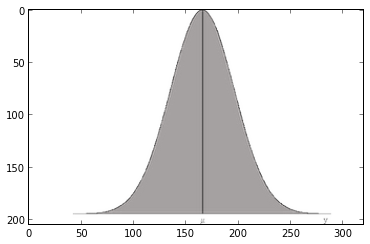
\includegraphics[width=0.7\textwidth]{dagilimlar2_files/dagilimlar2_fig_00.png}
\par
\end{center}
\end{codeoutput}
\end{codecell}
Mesela, Türkiye'deki 2000 yetişkinin kilosunu ölçün. Grafiğini alın,
kesinlikle yukarıdaki tepe şekli çıkacak. Ya da, 1000 kişinin boyunu
ölçün, aynı tepe şekli. Keskin nişancının hedefe attığı kurşunların
hedefe gelişini en iyi 12 en kötü 1 olmak üzere ölçün, sıklık grafiğini
alın. Gene aynı tepe şekli!

Nasıl oluyor bu iş?

Açıklama için, normal dağılım eğrisinden bahsetmemiz gerekecek.

Not olarak düşelim: Sıklık grafiği, X sayısının ne kadar çıktığını
sayıp, Y ekseni üzerinde bu sayıyı X'e tekabül ederek kolon olarak
göstermeye denir. Mesela, 60 kilo değeri 13 kere çıktı ise, X=60, Y=13
gibi bir kolon çizilecektir.

Normal Dağılım Eğrisi

Normal dağılımın olasılık kavramı ile yakın bağları var. Bu konuda ünlü
bir deney zar atma deneyidir. Mesela, elimizde tek bir zar olsun, ve bu
zarı arka arkaya atalım. Sabrımız yeterse 1000 kere atalım. Sonuçta,
sıklık grafiği eşit bir dağılım gösterecektir. (Zar tutmuyorsanız :) )

Bunun sebeplerini anlamak zor değil. Her zar atış olayı birbirinden
bağımsız, ve her sayının üstte gelme ihtimali birbirine eşit olduğu için
(1/6), her sayıdan eşit miktarda gelecektir. Tabii bunun için deneyin
birçok kere tekrarlanması gerekiyor.

Fakat, bir yerine 2 zar atalım. Hatta hatta, 4 zar atalım, ve bu sefer
sıklık grafik hanesine yazmadan çıkan sayıları önce toplayalım. Bu çıkan
toplamın sıklık grafiğini alalım.

İşte bu sıklık grafiği göreceğiz ki, önceden bahsettiğimiz tepe
grafiğine yaklaşıyor. Ne kadar çok zar atarsanız, bu benzerlik o kadar
daha fazla olacaktır.

Bunun sebebi de aslında basit: 1..6 arası sayıların tek bir zardan gelme
olasılığı aynı, evet. Fakat toplamlara gelince, mesela iki zarlı
örnekte, 10 sayısının olasılığı 2 sayısından daha yüksek. Çünkü, 10
sayısını 5-5, 4-6 ya da 6-4 ile alabiliyoruz. 2 sayısı sadece 1-1 ile
geliyor.

Buradan şu sonuç cıkabilir: Eğer doğada ölçtüğümüz bir kavramın
oluşmasında birden fazla etken var ise, o ölçümlerin sıklığı her zaman
tepe şekli ile olacaktır.

Fakat, daha da gizemli olan bir olay şudur; Sabit olan bir şeyi
ölçtüğümüzde (yaptığımız hatalar sonucu) çıkan grafiğin bile tepe
şekilli olması! Yani, doğru dürüst hata yapmak bile elimizde değil gibi
gözüküyor\ldots{} Bunun tabii ki olasılık açıklamaları olacaktır.
İzlediğimiz matematikçilerden bu en son konuda net bir açıklama
alamadık.

Simulasyon

Eğer bu kavramları simulasyon ortamında göstermek istersek, Python ile
bunu yapabiliriz.

İlk önce, Random.org sitesinden rasgele sayı üretip bilgiyarımıza
kopyalacağız. Bahsettiğimiz site, kimsenin kullanmadığı radyo
kanallarından atmosfer gürültüsü dinleyip, bu gürültüleri sayısal değere
çevirerek rasgele sayı üretiyor.

Gerçek rasgele sayı üretmek pek kolay bir iş değil. Her ne kadar
bilgisayarınızda rasgele sayı üreten birçok algoritma olsa bile, bu
algoritmalar belli bir sayı üretiminden sonra kendini tekrar etmeye
başlıyorlar. Gerçek rasgele sayılar için muhakkak dış bir kaynağa
bağlanmak gerekiyor.

Gösterimiz için, rasgele sayıları üretip, bir dat dosyasına koyuyoruz.
Python ile bu sayıları okuyup, ilk önce teker teker sayıların sıklık
grafiğini, ondan sonra sayıları üçer üçer toplayıp, onların grafiğini
alıp göstereceğiz. Aşâğıda bu iki grafiği bulabilirsiniz.

\begin{codecell}
\begin{codeinput}
\begin{lstlisting}
A = loadtxt('rasgele.dat');
hist(A, 50);

\end{lstlisting}
\end{codeinput}
\begin{codeoutput}
\begin{center}
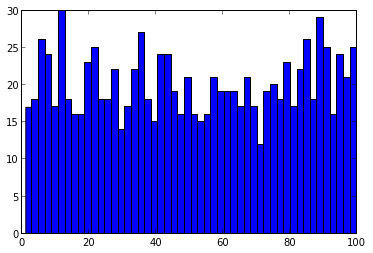
\includegraphics[width=0.7\textwidth]{dagilimlar2_files/dagilimlar2_fig_01.png}
\par
\end{center}
\end{codeoutput}
\end{codecell}
\begin{codecell}
\begin{codeinput}
\begin{lstlisting}
A = loadtxt('rasgele.dat');
B = []

i = 1;

while (i < 998):
  toplam = 0
  s = A[i]
  toplam = toplam + s
  s = A[i+1]
  toplam = toplam + s
  s = A[i+2]
  toplam = toplam + s
  B.append(toplam/3)
  i = i + 3

hist(B, 50);


\end{lstlisting}
\end{codeinput}
\begin{codeoutput}
\begin{center}
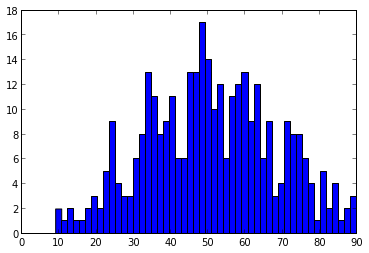
\includegraphics[width=0.7\textwidth]{dagilimlar2_files/dagilimlar2_fig_02.png}
\par
\end{center}
\end{codeoutput}
\end{codecell}

\end{document}
